This research follows an experimental framework aimed at comparing
the performance of classical and quantum transformer models in
natural language processing tasks. The study focuses on sentiment
classification, evaluating the accuracy of predictions made by both
classical transformers and hybrid classical-quantum transformers. In
the quantum model, classical linear layers were replaced with
\acrfull{VQC}, integrating quantum computation
into the standard transformer architecture. Two
types of transformer models were developed in this study: one with
embedding and positional encoding layers embedded within the
transformer, and another without these layers, requiring external
encoding through the pre-trained \gls{BERT} model.

Both models were trained and evaluated using identical datasets,
allowing for a fair performance comparison based on a metric called
accuracy. This approach was designed to explore the
potential advantages of quantum transformers over classical models in
terms of performance and computational efficiency, while also
considering different encoding methods.

\section{Data Collection}
\label{sec:data_collection}
Publicly available datasets from the Hugging Face library were
utilised to train and evaluate our transformer models.
The datasets used were carefully selected for their diversity in
sentiment analysis tasks and their scale, allowing robust model
performance testing. Below is a detailed overview of the datasets:

\begin{itemize}
  \item \textbf{IMDb Dataset}:
        This dataset~\cite{imdb_dataset} consists of 50,000 movie reviews
        and is designed for
        binary sentiment classification, with 25,000 reviews allocated
        for training and 25,000 for testing. The goal is to predict the
        polarity of reviews—either positive or negative—based on the
        text, making this dataset ideal for natural language processing
        and text analytics.

  \item \textbf{Amazon Polarity Dataset}:
        The Amazon Polarity dataset~\citep{yelp_amazon_dataset} contains
        approximately 35 million
        product reviews sourced from Amazon. Reviews are labelled as
        negative (ratings of 1 or 2) or positive (ratings of 4 or 5),
        with ratings of 3 excluded. The dataset provides 1,800,000
        training samples and 200,000 test samples for each class. Due to
        the large size of the dataset, it was sampled down to 600,000
        reviews to make it manageable for storage.

  \item \textbf{Yelp Reviews Polarity Dataset}:
        Derived from the 2015 Yelp Dataset Challenge, this
        dataset~\citep{yelp_amazon_dataset}
        consists of 1,569,264 review samples, where star ratings of 1 and
        2 are labelled as negative, and reviews rated 4 and 5 as
        positive. It includes 280,000 training samples and 19,000 test
        samples per class. Similar to the Amazon Polarity dataset,
        Yelp reviews were sampled down to 600,000 reviews for storage reasons.
\end{itemize}

\subsection{Data Preprocessing}
\label{subsec:data_preprocessing}
We utilised two distinct transformer models: one with an internal
embedding and positional encoding layer, and another without these
layers, requiring external encoding.

For the transformer model that includes an embedding layer, the IMDb
dataset was preprocessed using the torchtext library. The vocabulary
was built by tokenising the text with a basic English tokenizer and
creating a vocabulary index list from the dataset. The vocabulary
size was capped at 50,000 to ensure efficient memory usage during
training. Special tags such as \textlangle unk\textrangle\xspace
for unknown tokens and \textlangle pad\textrangle\xspace for
padding were added to the vocabulary. Once the vocabulary was
established, all words in the document were converted to their
respective indices from the vocabulary, preparing the dataset for
input into the transformer model.

For the transformer model without an embedding layer, the pre-trained
\gls{BERT} tokenizer from the Hugging Face transformer library was used to
tokenise the Amazon Polarity and Yelp datasets. Given the large size
of these datasets, they were sampled down to 600,000 entries to
manage memory usage. After tokenisation, the pre-trained \gls{BERT} model
was used to encode the words into 768-dimensional word embeddings.
The preprocessed datasets were then encoded and saved in tensor
format, with approximately 800GB of memory required to store these
tensors in the \acrshort{UWA} \gls{IRDS}. Since
the embeddings are fixed at 768 dimensions, further dimensionality
adjustments are handled later in the pipeline of the model. Further
sampling reduced the datasets to 300,000 entries for experiments.

This preprocessing ensured that the datasets were ready for input
into the respective transformer models, maintaining consistency in
text encoding across experiments.

\section{Implementation Details}
\label{sec:implementation_details}
The implementation of the transformer models involved several
technical steps to ensure compatibility between the classical and
quantum components and to handle the different preprocessing
requirements of each model.

For the transformer model with internal encoding layers, the
torchtext library was employed to manage tokenisation and vocabulary
creation. Text was first tokenised into word indices, which were
subsequently embedded using the built-in embedding layer of the model. The
integral positional encoding was automatically applied to the
embeddings, ensuring that sequence information was preserved. This
model adhered to a more traditional deep learning framework, where
data preprocessing and model operations were seamlessly integrated.
The inclusion of these encoding layers enabled the model to process
raw text data directly, without requiring any external encoding steps.

In contrast, the second transformer model relied on external
preprocessing. The text data was tokenised using the pre-trained \gls{BERT}
tokenizer, and the resulting tokens were passed through the \gls{BERT}
model to generate 768-dimensional embeddings. These embeddings were
then fed into the transformer model, ensuring that the input was in a
structured format suitable for further processing, even in the
absence of internal embedding layers. This architecture facilitated
experimentation with external encoding methods and allowed for
analysis of their impact on model performance.

\begin{figure}[ht]
  \begin{center}
    \subfloat[Quantum Transformer Architecture]{
      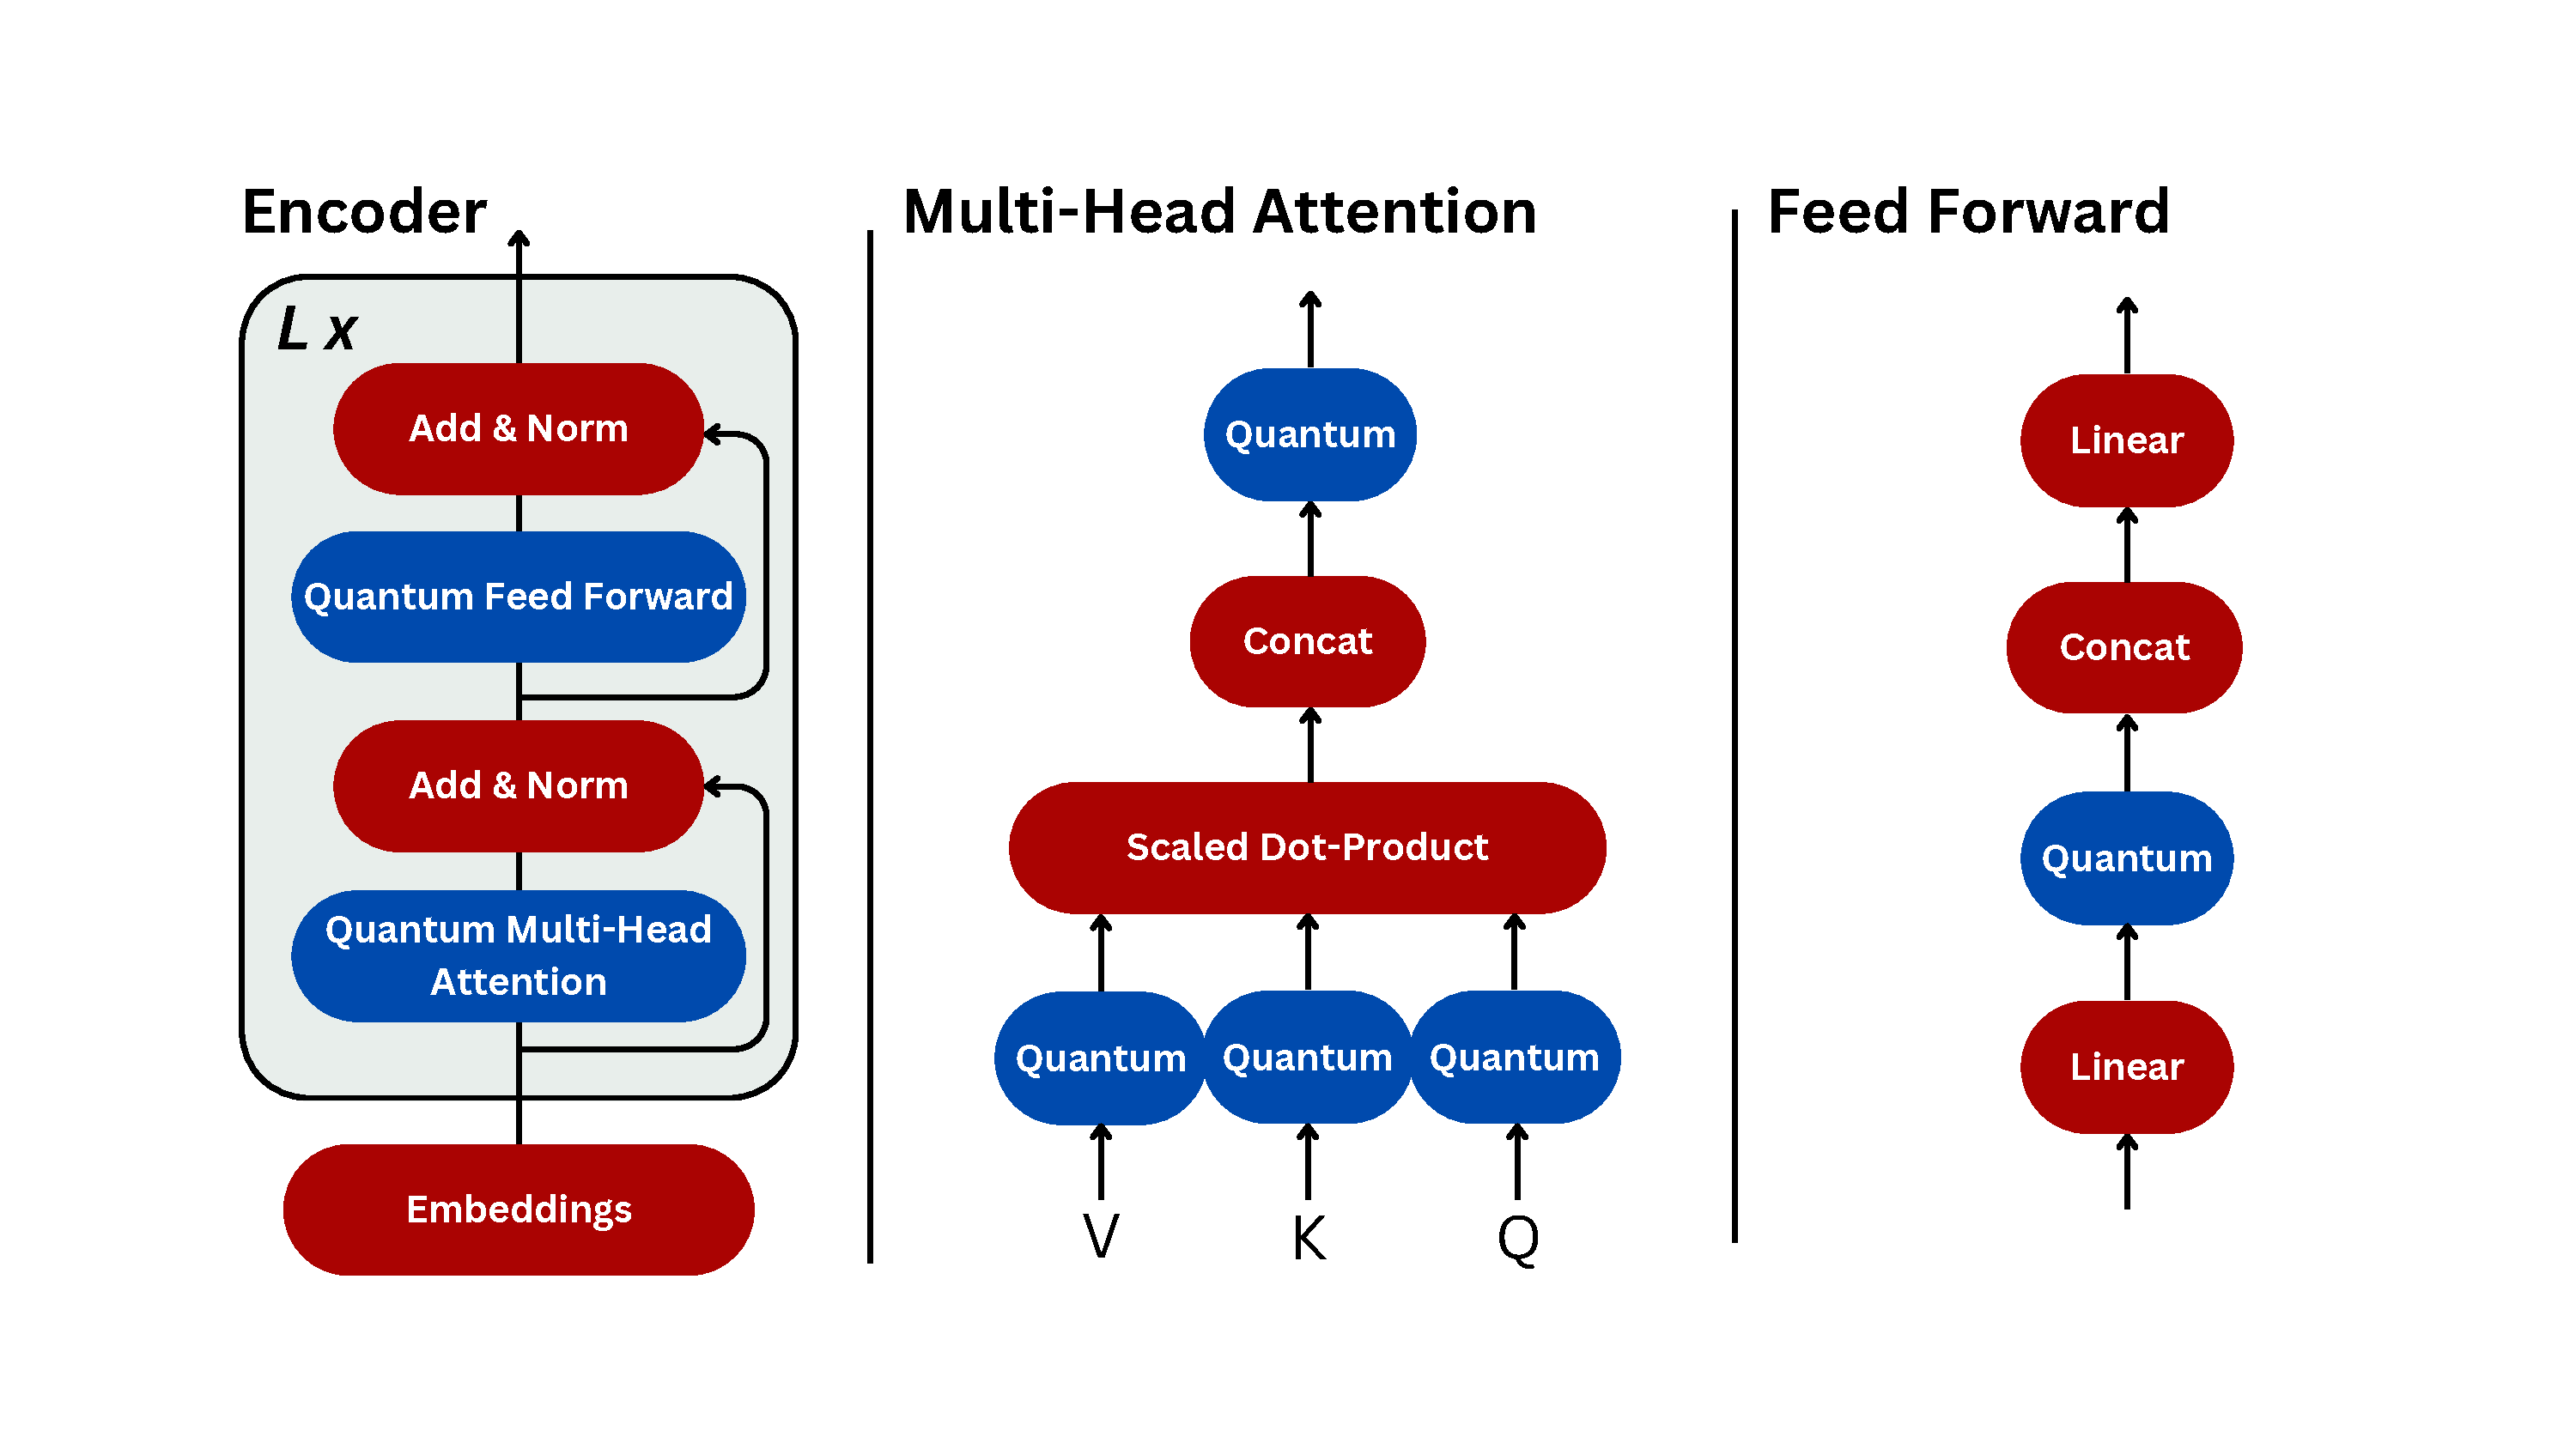
\includegraphics[width=0.98\textwidth]{img/quantum_transformer.pdf}
    }
  \end{center}
  \vspace{-0.5cm}
  \caption{An overview of the quantum transformer. The red components
    represent classical elements, including the embeddings, linear
    layers, and parts of the feedforward and attention mechanisms.
    The blue components denote quantum circuits, where quantum
    multi-head attention and quantum feedforward layers are
    integrated. Specifically, the classical linear layers are
    replaced by \gls{VQC}, which process the word embeddings within
    the quantum sections of the model. The
    illustration of the Transformer Encoder was inspired
    by~\citet{disipio2021dawn}.}
  \label{fig:qt_architecture}
\end{figure}

For the quantum transformer, the classical linear layers were
replaced by \glspl{VQC}, as illustrated in
Figure~\ref{fig:qt_architecture}. These circuits were constructed
using the Pennylane framework. The quantum circuits processed the
word embeddings, with an encoder used to adjust the dimensionality of
the embeddings to match the input size constraints of the quantum
circuits. Various encoding methods, including amplitude encoding and
angle encoding, were employed to translate classical data into
quantum states. For models using amplitude encoding, which compresses
\(2^n\) features down to \(n\) features, a decoder was needed to
decompress the features for the next layer. The basic \gls{VQC}
consisted of a single layer of parameterised gates followed by a ring
of \gls{CNOT} gates, introducing entanglement between qubits. The
strong \gls{VQC} increased the complexity, incorporating three layers
of parameterised gates followed by a ring of \gls{CNOT} gates. This
layering enhanced the expressibility of the model, allowing it to
capture more complex relationships in the input data.

There are also configurations that can be set within the quantum
circuits. For angle encoding, the rotation gate can be chosen from
\(R_x\), \(R_y\), and \(R_z\), depending on the desired rotation
axis. The basic and strong \glspl{VQC} are templates provided by
Pennylane. In the case of the basic VQC, the parameterised rotation
gates can be selected as \(R_x\), \(R_y\), or \(R_z\), giving
flexibility in the choice of rotational operations. However, for the
strong VQC, the parameterised gates are fixed to a sequence of
\(R_z\), \(R_y\), and \(R_z\) gates, which cannot be altered. The
only adjustable component in the strong VQC is the choice of the
two-qubit control gate, where options such as \gls{CNOT}, CZ,
or other controlled gates can be applied.

Finally, the expectation values of the Pauli-Z for all qubits are measured.
Measuring in Pauli-Z corresponds to measuring in the
computational basis (i.e., \( \ket{0} \) and \( \ket{1} \)), which
allows us to interpret the results classically. Although other
measurements, such as Pauli-X, are possible, which measure in the \(
\ket{+} \) and \( \ket{-} \) basis, we focus on Pauli-Z measurements
as they directly reflect the classical binary outcomes needed for
further processing in the model.

Both models were trained and evaluated on identical datasets, with
the same training configurations, including learning rates and batch
sizes. The evaluation focused on comparing the performance of the models
using accuracy metrics. By using the
same datasets and training conditions, the study provided a fair
comparison between the classical and quantum transformer models.
Simulated quantum environments were employed for the quantum model
experiments, using Pennylane and TensorCircuit to run
simulations on classical hardware.

\section{Setup}
\label{sec:setup}
The experiments were conducted in a \gls{HPC} environment using two
types of GPU clusters, depending on the availability of the clusters,
to train and evaluate both classical and quantum transformer models.
The following describes the computational environment:

\begin{itemize}
  \item \textbf{Hardware}: Two different types of GPU nodes were
        utilised from \gls{UWA} cluster:
        \begin{itemize}
          \item \textbf{Large GPU Nodes}: Dual Intel Xeon CPUs (36 cores
                total @ 3.1GHz), 768GB RAM, and Dual NVIDIA 32GB V100 GPU cards.
          \item \textbf{Medium GPU Nodes}: Dual Xeon CPUs (28 cores @
                2.0GHz), 256GB RAM, and 4 NVIDIA 16GB P100 GPU cards.
        \end{itemize}
  \item Only one GPU was used per experiment. This limitation was
        necessary due to Pennylane's own parallelisation mechanisms,
        which are unstable and prone to conflicts with PyTorch’s parallelisation.
        Both GPU nodes were configured to use CUDA 12.4.

  \item \textbf{Software Stack}: The following software stack was used
        for model development and experimentation:
        \begin{itemize}
          \item \textbf{Python}: Python 3.11.8 was used as the core
                language for model development and experimentation.
          \item \textbf{Jupyter Notebook}: All experiments were conducted
                and documented using Jupyter Notebooks for interactive model
                training and evaluation.
          \item \textbf{Conda}: Conda was used as the package manager for
                creating isolated environments with the necessary
                dependencies for both classical (PyTorch, TensorFlow) and
                quantum (Pennylane, TensorCircuit) frameworks.
        \end{itemize}
\end{itemize}

To ensure that all experiments were reproducible, several measures
were implemented. First, all models were seeded, ensuring that the
same random initialisations and conditions were applied across
different experiments. This enabled reproducibility when using the
same hardware and software configurations, ensuring consistency in
the behaviour of the model.

Additionally, intermediate results, such as model checkpoints and
partial outputs, were saved at various stages throughout the training
process. This approach allowed for consistent tracking of progress
and made it easier to reproduce experiments if needed. Saving
intermediate outputs also helped resume training from checkpoints
without having to restart from the beginning.

Lastly, Conda was used to manage the computational environment,
ensuring that dependencies remained consistent across experiments. By
isolating environments, potential issues related to version conflicts
or software updates were avoided, maintaining a stable environment
for the duration of the project.
